\subsubsection{Ciclo de vida}
    El ciclo de vida de los mixomicetos es muy complejo, sin embargo, un mixomiceto t\'ipico
        tiene un ciclo de vida que se puede dividir en dos etapas distintas, las cuales son:
        el plasmodio y uno o m\'as cuerpos fruct\'iferos.\cite{Stephenson1994}
    \vskip 0.5cm
    % Parrafo 5
    La secuencia de eventos que ocurren durante el ciclo de vida de un mixomiceto t\'ipico comienza con una espora 
        microsc\'opica que se form\'o dentro de y luego fue liberada de uno de los cuerpos fructiferos caracter\'isticamente 
        producidos por los mixomicetos. Bajo condiciones favorables, la espora germina para producir de uno a cuatro protoplastos haploides sin pared
        celular, denominados gametos. Estos son liberados a trav\'es de un peque\~no poro que se forma en la pared de la espora aunque tambi\'en pueden resultado 
        de la espora abri\'endose.
    \vskip 0.5cm
    % Parrafo 6
    Algunos protoplastos son flagelados cuando se liberan, mientras que otros son ameboides. Estos \'ultimos a veces pueden desarrollar flagelos despu\'es de un 
        corto per\'iodo de tiempo o, en algunos casos, simplemente permanecer ameboides. Las c\'elulas flageladas se llaman c\'elulas enjambre, mientras que las 
        c\'elulas no flageladas se llaman mixoamoebas. Las mixoamoebas y las c\'elulas enjambre son interconvertibles, y la forma particular en la que existe una 
        c\'elula dada depende aparentemente en gran medida de la disponibilidad de agua libre en su entorno inmediato. En presencia de agua libre, la forma 
        flagelada tiende a predominar, mientras que bajo condiciones de escasez de agua, las mixamoebas sin flagelos son m\'as comunes.\cite{Stephenson1994}
    \vskip 0.5cm
    % Parrafo 7
    Las mixamoebas y las c\'elulas enjambre se dividen en dos, y cuando las condiciones no son buenas, 
        las mixamoebas pueden convertirse en estructuras inactivas llamadas microquistes, que les ayudan a sobrevivir 
        por mucho tiempo. Cuando dos de estas c\'elulas se juntan, forman un cigoto, que puede ser ameboide o flagelado, pero 
        eventualmente se convierte en ameboide y crece para convertirse en un plasmodio, una estructura grande con muchos n\'ucleos 
        pero que funciona como una sola c\'elula. Si las condiciones se vuelven dif\'iciles, como por la falta de agua o fr\'io, el plasmodio 
        se puede transformar en un esclerocio, una forma resistente que puede volver a convertirse en plasmodio cuando las condiciones 
        mejoren. En invierno, es posible encontrar esclerocios debajo de la corteza de troncos y tocones en descomposici\'on.
    \vskip 0.5cm
    % Parrafo 8
    El ciclo de vida de los mixomicetos se puede observar en la figura \ref{fig:MixomicetoCicloVida}, en donde: 
    \renewcommand{\labelenumi}{{\Alph{enumi}})} 
    \begin{enumerate}
        \item Espora 
        \item Germinaci\'on de la espora
        \item Etapa unicelular, que es o una mixoamiba (izquierda) o una c\'elula enjambre (derecha).
        \item Microquiste
        \item Fusi\'on de dos mixoamoebas o c\'elulas enjambre para producir solo una c\'elula.
        \item Fusi\'on de dos mixoamoebas o c\'elulas enjambre para producir solo una c\'elula.
        \item Cigoto
        \item Plasmodio temprano
        \item Esclerocio 
        \item Plasmodio maduro
        \item Comienzo de la esporulaci\'on 
        \item Cuerpos fruct\'iferos maduros con esporas a\'un encerradas
    \end{enumerate}
    \begin{figure}[h]
        \centering
        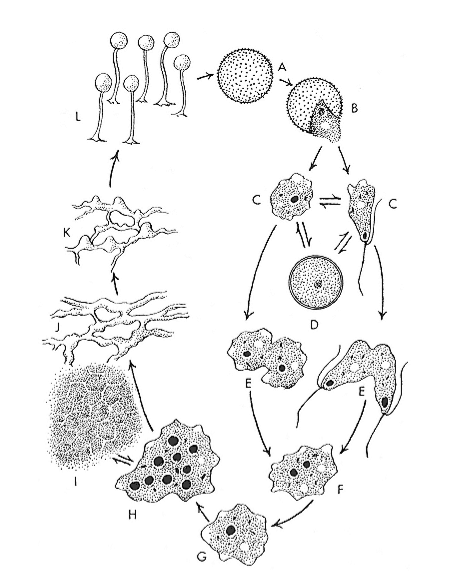
\includegraphics[width=0.5\textwidth]{./images/marco_teorico/Physarum/mixomiceto_ciclo_vida.png}
        \caption{Ciclo de vida de los mixomicetos, extraido de "Myxomycetes: A Handbook of Slime Molds" de Stephenson y Stempen \cite{Stephenson1994}.}
        \label{fig:MixomicetoCicloVida}
    \end{figure}
    \vskip 0.5cm
    % Parrafo 8
    Si desea profundizar en el tema, puede consultar el libro "Myxomycetes: Biology, Systematics, Biogeography, and Ecology" de Rojas \cite{Rojas2017}.
    \vskip 0.5cm
    \clearpage